%\documentclass{article}
\documentclass{chi2009}
\usepackage{times}
%\usepackage{uist}
\usepackage{url}
\usepackage{graphics}
\usepackage{color}

% \newcommand{\want}[1]{{[\color{blue} WANT: #1]}}
% \newcommand{\todo}[1]{{[\color{blue} TODO: #1]}}
% \newcommand{\idea}[1]{{[\color{blue} IDEA: #1]}}
% \newcommand{\node}[1]{{[\color{blue} NOTE: #1]}}

\newcommand{\want}[1]{}
\newcommand{\todo}[1]{}
\newcommand{\idea}[1]{}
\newcommand{\node}[1]{}




\begin{document}

% --- Copyright notice ---
\conferenceinfo{UIST'09}{October 4-7, 2008, Victoria, BC, Canada}
\CopyrightYear{2009}
\crdata{x-xxxxx-xxx-x/xx/xxxx}

% Uncomment the following line to hide the copyright notice
\toappear{}
% ------------------------

\bibliographystyle{plain}

\title{Exposing Disputed Statements on the Web}

%%
%% Note on formatting authors at different institutions, as shown below:
%% Change width arg (currently 7cm) to parbox commands as needed to
%% accommodate widest lines, taking care not to overflow the 17.8cm line width.
%% Add or delete parboxes for additional authors at different institutions. 
%% If additional authors won't fit in one row, you can add a "\\"  at the
%% end of a parbox's closing "}" to have the next parbox start a new row.
%% Be sure NOT to put any blank lines between parbox commands!
%%

\author{
\parbox[t]{9cm}{\centering
	     {\em Author names removed for blind review}\\
}
}

\maketitle

%RULE: Don't cite media reports unless I have to

\abstract
We present Think Link, a browser extension that aims to let users see when the information they are reading presents only one side of a disputed issue. As the user browses the web, Think Link highlights snippets of text that make claims that conflict with information on other web sites. If a user clicks on such a disputed claim then Think Link will show them an argument graph showing the best evidence for and against the claim being true, as determined by other users of Think Link.

\classification{H5.2 [Information interfaces and presentation]:
User Interfaces. - Graphical user interfaces.}

\terms{Design, Human Factors}

\keywords{CSCW, Sensemaking, Annotation, Argumentation, Web}


\tolerance=400 
  % makes some lines with lots of white space, but 	
  % tends to prevent words from sticking out in the margin

\section{INTRODUCTION}

The web provides users with a huge number of pages that they can read, but extracting accurate and balanced information from these pages can be difficult. Not everything on the web is accurate~\cite{Mintz2002,Neumann2003,Resnik1998,Zhou2004} and many web sites present only one side of a contentious issue~\cite{Herman2002,Gentzkow2007}. If a user is to form a rounded opinion about a topic then they will need to either stick to sources that they trust or spend time looking for evidence on other web sites that supports or opposes what they read. Even if a user tries hard to research every topic they read, they can still get caught out by beliefs that they had not realized were disputed.


In this paper we present Think Link, a tool helps users discover when information they read conflicts with information on other web sites, and shows users the best sources that provide alternative points of view. When Think Link is used as a browser plugin it will highlight text that makes a disputed claim. If a user clicks on such a highlighted snippet then Think Link presents the user with an argument graph that shows the best evidence for and against the claim, as judged by other users of Think Link (Figure~\ref{claimview}). The argument graph contains links to snippets of text on other web sites that express conflicting or supporting points of view.

\begin{figure}[tb]
	\begin{center}
	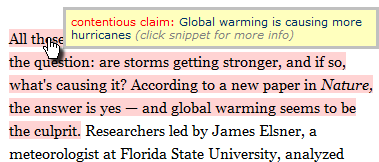
\includegraphics[width=5cm]{../screenshots/highlight_crop.png}
	\caption{Think Link highlights snippets that make disputed claims}
	\label{highlight}
	\end{center}
\end{figure}


Think Link relies on users to identify disputed claims, to find appearances of these claims on web sites, and to vote for which snippets are most important. If a user is viewing a web page, they can identify disputed claims and useful evidence. Think Link will guide a user in finding existing claims that a snippet may be making and in connecting existing claims.

\begin{figure}[tb]
	\begin{center}
	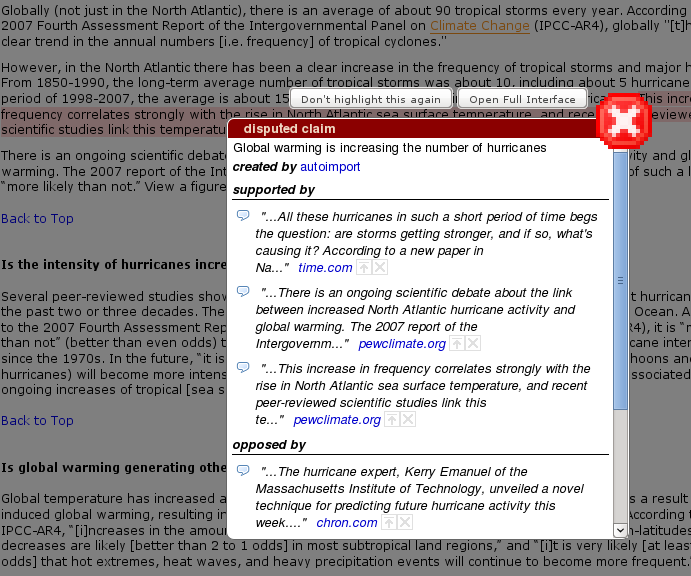
\includegraphics[width=5cm]{../screenshots/v2_popup_dim.png}
	\caption{Click on a claim to investigate evidence for and against it}
	\label{claimview}
	\end{center}
\end{figure}

\todo{Claim panel should have 'more' buttons}

Think Link is designed to cater to two distinct groups of people. Activists care strongly about particular claims that they disagree with and combine Think Link with a preferred search engine to find instances of these claims and mark them up so other users can see them. Sceptical readers install Think Link as a browser plugin so that they can see when things they read and disputed and find other links that present other points of view. A reader may of course be an activist for one issue and a sceptical reader for others.

The design of Think Link was guided by two user studies, in which we observed the behavior of users who fitted the roles of Activist or Sceptical Reader. 

\todo{Talk about automatically including all arguments from Snopes}.



% \begin{figure}[tb]
% 	\begin{center}
% 	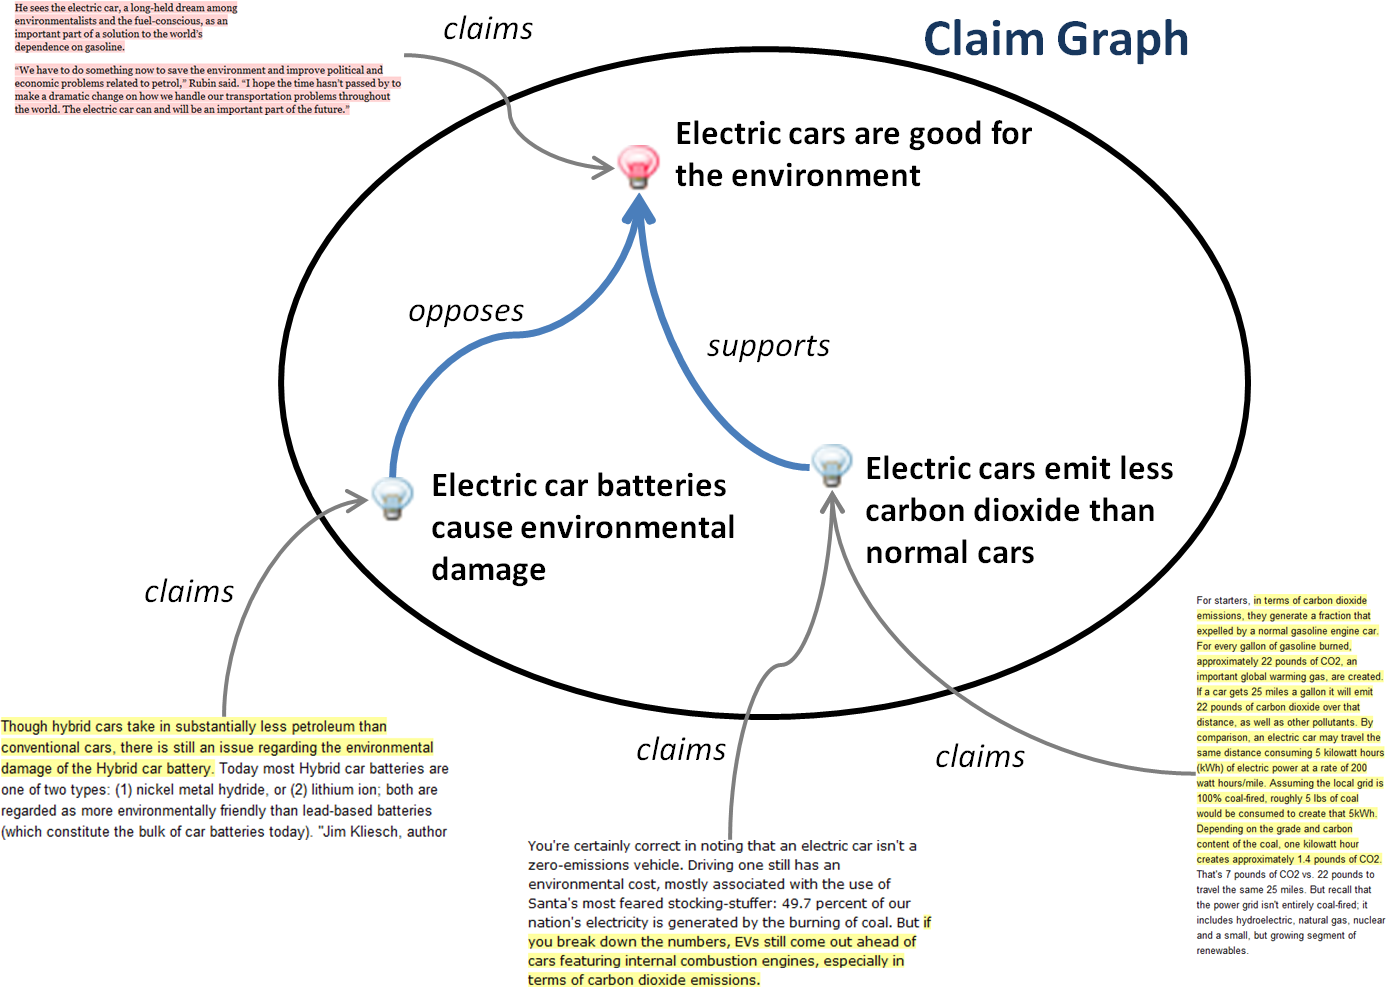
\includegraphics[width=7.7cm]{../screenshots/summary_graph.png}
% 	\caption{Think link connects claims to each other and to web snippets}
% 	\label{summarygraph}
% 	\end{center}
% \end{figure}


\section{Related Work}
\todo{Don't cite things that aren't relevant}

Think Link builds on work in several different areas. The argumentation structure influenced by IBIS~\cite{Rittel1973} tools such as gIBIS~\cite{Conklin1987a}; the idea of highlighting information that may not be trustworthy was previously applied to Wikipedia by Wiki-Trust~\cite{Adler2008}; the model of using a community to collect and filter information from a range of sources is influenced by tagging systems~\cite{Marlow2006}; and the idea of gathering up a collection of snippets from web pages has been used by clipping tools such as Internet Scrapbook~\cite{Sugiura1998}. 

What makes Think Link interesting is the way that it combines ideas from these different domains and applies them to the task of leading users towards information that conflicts with that which they read.

\subsection{Argumentation}

Think Link is an example of an Issue Based Information System (IBIS)~\cite{Rittel1973}. IBIS tools such as gIBIS~\cite{Conklin1987a}, Compendium~\cite{Selvin2001}, Collabatorium~\cite{Klein2007}, Zeno~\cite{Gordon1997}, and Cohere~\cite{Shum2008} model discouse as a graph of connected ideas. While the graph structure varies between tools, most tools allow one to mark an idea as supporting or opposing another idea, and allow one to mark an idea as addressing an issue. Some tools, such as Collabatorium~\cite{Klein2007} and Cope It~\cite{Karacapilidis2006} structure an argument as a tree, while others such as Think Link, gIBIS~\cite{Conklin1987a} and Cohere~\cite{Shum2008} structure an argument as a graph, in which a single idea can support or oppose multiple other ideas.

Cohere is perhaps the tool most similar to Think Link. Cohere allows one to use snippets from web pages as evidence to support ideas in its argument graph and provides a Firefox plugin that makes it easier to grab snippets from pages that one browses. While Cohere and Think Link both connect an argument graph to the web, they do so in very different ways. In Cohere, a user attaches a web snippet to their idea in order to use it as evidence. By contrast, in Think Link, the main reason to connect a web snippet to an argument is to mark the snippet as contentious and encourage other readers of the snippet to look at the argument. 

ClaimSpotter~\cite{Sereno2005,Sereno2004} allows one to mark up a scholarly document with logical triples (subject, verb, object) describing interesting claims that are being made in the document. This semantic information can be used to connect claims in different documents and see when a logical claim in one document contradicts another. Entity Workspace~\cite{Bier2006} does something similar for intelligence documents.  

Think Link uses a relatively simple graph structure, similar to that of gIBIS~\cite{Conklin1987a}, allowing a claim to support, oppose, or be related to another claim. Cohere~\cite{Shum2008} extends this by allowing one to new link types marked with pro,con,or neutral polarity Toulmin~\cite{toulmin1958} proposes a more complex graph structure, that expresses warrants, data, qualifiers, and reservations. Verheij~\cite{Verheij1999} uses the Toulmin model to create an argumentation tool for lawyers. More complicated models such as Carneades~\cite{Gordon2007} have been used for artificial intelligence, where it is necessary to be more precise about the structure of an argument.

Think Link's argument visualization is influenced by the left-to-right layout of Cohere~\cite{Shum2008}. Compendium~\cite{Selvin2001} contains a number of other visualizations of argument graphs. Mess Maps~\cite{Horn2007} present an alternative view in which an argument is divided into different sectors, each of which presents the argument from a different frame of discourse (e.g. policy maker vs industrialist vs environmentalist).

Isenmann and Reuter~\cite{Isenmann1997} identify a number of problems with the IBIS model, which they argue are reasons why it has not achieved widespread use. We believe that while the problems they observe are important when an IBIS tool is being used for conflict modelling and resolution they are less of a problem for a tool like Think Link that is designed primarily for conflict discovery. We do not expect users to use Think Link to create a detailed model of an argument and use this to reach consensus. Instead, our aim is that a user should use Think Link to discover when things they read are disputed, and easily find evidence for the other side.
\todo{Say more about this}.

When choosing an argumentation structure, there is an inherent trade-off between accurately modelling the structure of an argument and making the tool easy to use. For Think Link, we have tried to minimize the complexity of the model, and thus adopted a very simple pro/con/netural link model. The idea here is not so much to present the detailed logical structure of an argument as to show a user what sources they should look at when forming an argument for or against a claim.

% \subsection{Open Hypermedia}
% 
% 
% \todo{Talk about other hypertext systems - mention arguments integrated into documents an old idea and talk about open hypermedias}

% TRELLIS
% 
%  gIBIS~\cite{Conklin1987} and other IBIS~\cite{Rittel1973} such as ZEN
% 
% Cohere~\cite{Shum2008} is probably the tool most similar
% 
% 
% 
% Cohere~\cite{Shum2008}. Compendium~\cite{Selvin2001}. Cope it~\cite{Karacapilidis2001}. AIF~\cite{McGinnis2007} and ArgDF~\cite{Rahwan2007}. IBIS~\cite{Rittel1973}. gIBIS~\cite{Conklin1987}. IBIS problems~\cite{Isenmann1997}. ClaimSpotter~\cite{Sereno2005,Sereno2004}. ClaiMaker~\cite{Uren2003}. Video Annotation~\cite{Diakopoulos2008}. Collabatorium~\cite{Klein2007}, for Global Warming~\cite{Malone2007}. Lawyer argument model~\cite{Verheij1999}. Toulmin model~\cite{Toulmin1958}. Zeno~\cite{Gordon1997}. Discoursium~\cite{Yetim2007}.
% Entity Workspace~\cite{Billman2007}. 
% Mess Maps and Resolution Mapping~\cite{Horn2007}.
% TRELLIS~\cite{Chklovski2005}.  
% People should define own link types~\cite{Wang1998}.
% 
% Hypertext systems such as Notecards~\cite{Halasz1988}.

\subsection{Checking Accuracy and Bias on the Web}

If one sees a claim on the web that one suspects might be untrue then one can look it up on Snopes\footnote{http://snopes.com} or FactCheck\footnote{http://factcheck.org}. Snopes is a database of urban legends that the site owners have investigated to determine whether they are true or not. FactCheck is a web site that investigates claims being made by US political parties and attempts to uncover the facts. Think Link's database automatically imports all contentious claims identified by Snopes.

NewsCube~\cite{Park2009} and MediaCloud\footnote{http://mediacloud.org} use statistics to help readers avoid media bias. NewsCube presents a user with articles on the same topic that have different biases. MediaCloud applies various statistical analyses to news sources so that a reader can see when different news sources associate different words with the same topic.

Several authors have investigated ways to make Wikipedia\footnote{http://wikipedia.org} more trustworthy. WikiTrust~\cite{Adler2008} highlights passages on wikipedia based on the likelihood that another user will change that text in the future --- recent edits by untrusted editors are marked as less trustworthy than old edits by trusted editors. Wiki Dashboard~\cite{Kittur2008} presents the reader of a Wikipedia article with a visualization that shows them how it has been edited in the past and lets them see graphically how contentious the topic is. Wiki Scanner\footnote{http://wikiscanner.virgil.gr} finds Wikipedia edits that have been made by people with an interest in spreading misinformation (e.g. people from a company editing pages about that company).

% 
% 
% NewsCube~\cite{Park2009}.
% Wikipedia fixes Vandalism~\cite{Viegas2004}.
% Trustworthiness~\cite{Gil2006}.
% WikiTrust~\cite{Adler2008}. Wiki Dashboard~\cite{Kittur2008}.
% Wiki Scanner\footnote{http://wikiscanner.virgil.gr}.
% SourceWatch\footnote{http://sourcewatch.org}, Snopes\footnote{http://snopes.com}, FactCheck\footnote{http://factcheck.org}.

\subsection{Annotating, Tagging, and Clipping}

Think Link is an example of an Open Hypermedia system~\cite{Bouvin2000}. Like other Open Hypermedia systems, Think Link allows users to lay an additional link structure over an existing hypertext document. Think Link differs from prior open hypermedia systems in its focus on revealing contentious arguments. While other systems such as HyperDISCO~\cite{Wiil1996} could be used to link a snippet to a contentious claim, they do not provide user interface support to make this easy.

\todo{Say how different from other Open Hypermedia link annotation systems}

Tagging Systems~\cite{Marlow2006,Golder2006} allow users to collect and organize information by associating it with an ad-hoc collection of tags. Notable tagging systems include del.icio.us\footnote{http://del.icio.us} which uses tags to organize web pages, and Flickr\footnote{http://flickr.com} which associates tags with photos. 

Annotation tools~\cite{Marshall1998} such as Annotea~\cite{Koivunen2001}, CritLink~\cite{Yee2002}, 

Some tagging and annotation tools also do clipping. Clipping tools such as Internet Scrapbook~\cite{Sugiura1998}, Hunter Gatherer~\cite{Schraefel2002}, ScratchPad~\cite{Gotz2007}, ClipMarks\footnote{http://clipmarks.com}, and Diigo\footnote{http://diigo.com} allow users to collect text snippets from web pages, tag them, and share them with friends. In many cases, a tagging or clipping system will also allow users who are looking at a tagged or clipped object to see the tags that other users have associated with it, or highlight the parts of a document that have been clipped.

Several tools allow users to annotate content that is considered to controversial. Videolyzer~\cite{Diakopoulos2008} allows users to annotate and comment on political videos with accompanying textual transcriptions. A user can mark up a section of video for bias, accuracy, or rhetorical technique. Comments can include references to external sources that back up the argument being made. SpinSpotter\footnote{http://spinspotter.com} allows a user to highlight snippets of text that contain spin or bias and either describe why the text is biased, or rewrite the text in an unbiased way. While SpinSpotter and Think Link share a goal of drawing user attention to biased or inaccurate information, they do so in a different way. SpinSpotter annotates a snippet with an annotation specific to that particular snippet of text, while Think Link treats a snippet as being an instance of a shared contentious claim, and links all snippets identified as making that claim to a shared graph node linking to other information about that claim.

\subsection{Augmented Web Navigation}

Several tools layer an alternative navigation graph over information on the web. TextRunner~\cite{Etzioni2008} and Idea Navigation~\cite{Etzioni2008} look for instances of subject-verb-object triples on web pages and connect these together as a graph in which objects are linked by statements made about them on different web pages. ScentHighlights~\cite{Chi2005a} highlights snippets of text on a web page that are related to topics that the user has said that they are intersted in. Kolak and Schillit~\cite{Kolak2008} detect cases where one book has quoted from another one, and use this to create links between books. This ``linking of quotations'' is similar in spirit to the linking of claims in Think Link. 

% Tagging~\cite{Marlow2006}. Tagomizer~\cite{Park2007}. Reasons for choices of tags~\cite{Sen2006}. Tagging Roles~\cite{Muller2008}. 
% 
% SpinSpotter\footnote{http://spinspotter.com}. ClipMarks\footnote{http://clipmarks.com}, Diigo~\footnote{http://diigo.com}, Stickis\footnote{http://stickis.com}.
% 
% How to Personalize the Web~\cite{Barrett1997}. 

% \subsection{Clipping}
% 
% ScratchPad~\cite{Gotz2007}. Internet Scrapbook~\cite{Sugiura1998}. Reverse Linking~\cite{Yesilada2007}. Hunter Gatherer~\cite{2002}. Dontcheva~\cite{Dontcheva2007a}.

% \subsection{Semantic Web}
% 
% Nobody is going to mark up their own web page as being wrong.

% \subsection{To discuss in the body}
% 
% Paraphrases~\cite{Chklovski2005}. Suggested formal paraphrases~\cite{Blythe2004}.
% Importance of Lurkers~\cite{Takahashi2003}
% Wikify~\cite{Mihalcea2007}. OpenCalais\footnote{http://opencalais.com}.

%\subsection{Automated Reasoning}
%
%Case-Based reasoning
%Sensemaking

%\subsection{Argumentation Graphs}
%Argumentation graphs express positions and arguments in a formal graph model as nodes and edges, respectively, and are typically used to make a decision or draw a conclusion about some issue. One example implementation is the {\it Zeno} argumentation framework~\cite{zeno}, designed for collaborative use in mediation systems to debate the quality of alternative solutions for a problem. In their object model of argumentation elements, based on Rittel's IBIS model~\cite{ibis}, example nodes include pro/con arguments, positions, preferences, comments, and decisions. Importantly, arguments are connected via {\it consequent} and {\it antecedent} edges, which are used to inform {\it choices}. The decision-making power of the argumentation graph follows from the traversal of argument relationships to enhance the depth and breadth of understanding about an issue. Our application similarly links claims as {\it supporting} and {\it opposing} other claims to allow users to develop a cohesive understanding of arguments.
%
%Traditional argumentation graphs are designed to solve a specific, isolated issue. Our application supports an ever-expanding set of topics, and arguments can form links between multiple topics. Users can consult the web of ideas directly to form an opinion about a particular issue, but they can also browse for new issues to explore. Opinions or decisions in our model don't have to be static: as the topic is expanded with more supporting and opposing evidence, users may alter previous viewpoints. Another advantage of our model is that the ability to explore claims' source-document evidence is built right into the navigation. Looking at an argument shows both its related argument as well as its supporting {\it snippets}, allowing the user to explore the evidence for himself. 

\section{The Think Link System}

Think Link is designed to be used in two different ways. Sceptical readers browse the web and wish to be alerted when information they read conflicts with information found on other web sites. Activists scour the web for web sites that make claims that they disagree with so that they can draw the attention of sceptical readers to claims that they disagree with. The same user may act as a sceptical reader sometimes and an activist at other times.

\subsection{Browsing the Disputed Web}

If a sceptical reader has installed the Think Link browser extension then Think Link will draw the users attention to text snippets that make or imply disputed claims by highlighting them in red (Figure~\ref{highlight}). If a user hovers their mouse over a highlighted snippet then Think Link will display a tooltip saying what the disputed claim is. If the user clicks on a highlighted snippet then Think Link will display a visualization showing the best evidence for and against the claim being true, as determined by the user community (Figure~\ref{claimview}). 

Since the purpose of a highlight is to alert the user to claims that they had not realized were contentious, there is little benefit in highlighting snippets that make claims that the user already realizes are contentious. A user can click the ``don't highlight this claim again'' button to tell Think Link that they are aware of the contentious nature of this claim and do not wish to be alerted about it again.

\todo{ignore button}
\todo{talk about the margin?}

\subsection{Exploring the Argument Graph}

\begin{figure}[tb]
	\begin{center}
	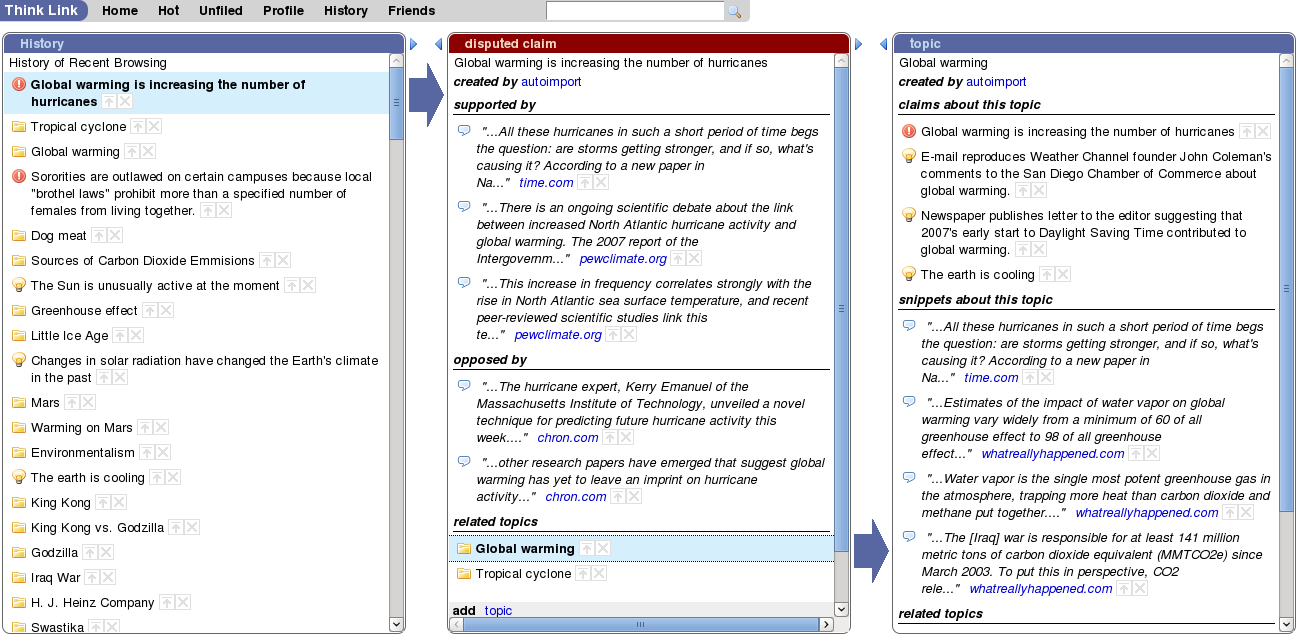
\includegraphics[width=8.5cm]{../screenshots/v2_panels.png}
	\caption{The claim graph consists of a series of linked panels}
	\label{panels}
	\end{center}
\end{figure}

Once a user has identified a claim that they are interested in, they can use Think Link's claim browser interface (Figure~\ref{panels}) to investigate the evidence for and against it, and to see what other contentious claims have been made about related issues. 

In our user studies, we found that users wanted to be able to investigate the evidence for and against a claim without having to navigate away from that claim. We thus created an interface that consists of a horizontal array of panels where each panel provides information about the item that is selected in the panel to its left. If a panel describes a disputed claim, then a user can investigate a particular piece of supporting evidence by clicking on it and looking at the information in the panel to the right. To emphasis the connection between the panels, the claim browser places an arrow next to each selected item, pointing to the panel that gives more information about that item.

\begin{figure}[tb]
	\begin{center}
	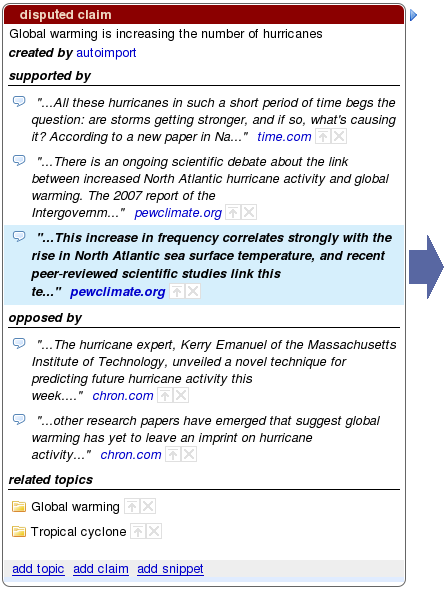
\includegraphics[width=6cm]{../screenshots/v2_panel.png}
	\caption{A claim panel presents information for and against a claim}
	\label{panel}
	\end{center}
\end{figure}


We found that it was important to allow the claim browser interface to be used in two different ways. When a user is browsing a web page and sees a disputed claim they want to be able to quickly see a small popup window giving evidence for a disputed claim without having to navigate away from the page~(Figure~\ref{claimview}); however if they are interested in the claim and want to investigate the evidence for a claim in more detail then the small popup interface is too small to easily view large amounts of information and so it is preferable to use a full-window interface. 

To preserve visual consistency, Think Link uses the same claim browser interface for the small popup interface as for the full-window interface. When used as a popup browser, the interface shows only one panel. Clicking on an item in the panel scrolls the display to the right to reveal a new panel in a manner similar to Apple's iPhone. If the user clicks the ``back'' button, the interface will quickly scroll left back to the previous panel.

\begin{figure}[tb]
	\begin{center}
	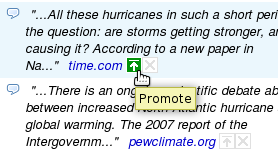
\includegraphics[width=6cm]{../screenshots/v2_vote.png}
	\caption{Voting buttons let users say which evidence is important}
	\label{voting}
	\end{center}
\end{figure}

%\todo{Key issue with hypertext was not talking about things that highlighted arguments?}

Think Link's claim graph is a variant of the IBIS~\cite{Rittel1973} model. There are four types of node: snippets, claims, topics, and users. A snippet is a region of text taken from a web page; a claim is a statement about the world or position that one can take on some issue; a topic is an issue or concept that a claim might relate to, and a user is a person who users Think Link. Nodes are connected together by typed, directed, links. There are three link types: supports, opposes, and relates-to. A claim can support,oppose, or relate-to another claim, a claim can relate-to a topic, and a topic can relate-to another topic. This is similar to the model used by gIBIS~\cite{Conklin1987} except that we don't distinguish between an argument and a position, and we allow a claim to simply relate-to another claim, rather than having to either support or oppose it.

Think Link uses topics to group together related claims. A topic be an issue that several claims are proposing solutions for, for example ``What should we do about global warming?''. Alternatively, it can be a thing that claims are about, for example ``Carbon Dioxide''. Think Link uses the list of page titles on Wikipedia as a seed-set for its topics.

The panel for a claim lists evidence that will help a user decide whether the claim is true. Evidence is categorized as either supporting, opposing, or being related-to the claim. The ``related-to'' category is used for evidence that does not fit neatly into one side of the argument. Evidence can either be a snippet that talks about that claim, or another claim whose truth would support the truth of this claim. 

The order in which evidence is displayed is determined by user voting. A user can vote for or against a particular piece of evidence by clicking on the voting button next to that item~(Figure~\ref{voting}). When a user looks at a list of evidence they will see first the things they voted for and then the other evidence ordered based on the number of votes it received from other users.

One danger in a voting system is that a large group of people will drown out the opinions of their opponents by voting down their opinions. Think Link uses several strategies to try to avoid this happening. Firstly, positive votes count for more than negative votes. Thus if two different groups are voting up their own evidence and voting down the opposing group's evidence, it is still likely that the opinions of both groups will be relatively prominent. Secondly, a piece of evidence only competes against other pieces of evidence on the same side of the argument, thus even if supporters of one side are voting up their own evidence, this will not push down evidence on the other side. Of course, these techniques only work to a limited extent, and so we expect that editorial moderation may be needed for highly controversial topics, as it is in Wikipedia.

\todo{Talk about searches}
\todo{Cite work on collaborative filtering}
\todo{Mention the sidebar?}

% If the current page contains snippets then a tab appears in the top left corner of the window. The tab contains a light bulb icon whose color changes according to the nature of the snippets on the page (Figure~\ref{bookmark_icons}) - red if a snippet contains a contentious claim. This allows a user to quickly tell if a page contains something of interest without having to scroll through the whole page. Clicking on the tab opens the margin. The margin provides a summary of all the interesting claims that users have identified on the current page and is designed to mimic the traditional margin notes that readers often write on physical documents~\cite{marginalia}. To emphasize the connection between a margin note and its associated snippet, each margin note is aligned vertically with its snippet and the snippet is highlighted more strongly when the user mouses over the associated margin note. 

\subsection{Campaigning on the Disputed Web}

If a user has installed the Think Link browser extension then they can create a snippet from text on a web page by selecting the text and selecting either ``This is disputed'' or ``This is interesting'' from the context menu. A user selects ``This is disputed'' if they believe that readers of that snippet should be alerted of the fact that a claim that that snippet is making or implying is disputed. A user selects ``This is interesting'' if they believe that the snippet contains useful information that would be useful to readers investigating a disputed claim. 

\begin{figure}[tb]
	\begin{center}
	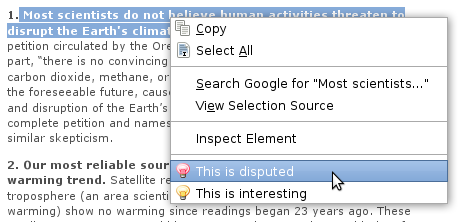
\includegraphics[width=6cm]{../screenshots/v2_snipmark.png}
	\caption{Use the context menu to mark a new snippet}
	\label{createprocess}
	\end{center}
\end{figure}

Think Link does not require that a user associate a snippet with a snippet at the point at which they create it. Instead, Think Link encourages a user to associate snippets with claims and topics ``in bulk'' using the claim browser interface, after they have gathered many snippets. One anticipated usage scenario for Think Link is an activist user who users a search engine to find a large number of snippets that make a clam that the user disagrees with. In this case, the user can save time by attaching all the snippets to the same claim together, rather than having to pick the same claim for each one.

Think Link provides three ways for a user to associate a claim with a snippet:

\begin{description}
\item[Claim first:] If a user navigates to a claim and clicks the ``add snippet'' button, Think Link will suggest unattached snippets that the user created recently and that are textually similar to the wording of the claim or other snippets currently attached to the claim (Figure~\ref{snipclaim}). A user can attach a suggested snippet to the claim by clicking on icons representing ``supports'', ``opposes'', or ``relates to'' link types. If Think Link does not suggest the right snippets then Think Link can guide the suggestions by entering keywords into the text box above the suggestion list.

\begin{figure}[tb]
	\begin{center}
	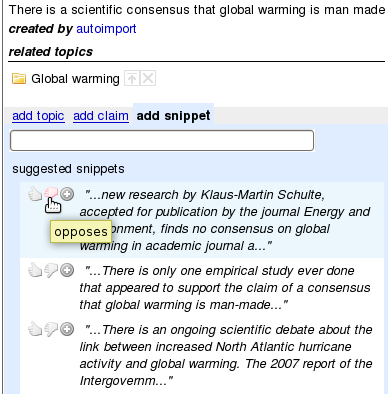
\includegraphics[width=6cm]{../screenshots/v2_sugsnippet.png}
	\caption{Claim first: Pick unfiled snippets to attach to a claim}
	\label{snipclaim}
	\end{center}
\end{figure}

\item[Snippet first:] If a user selects the ``unfiled'' tab at the top of the claim browser then Think Link will show a list of all the snippets that they have marked but not yet associated with a claim or a snippet (Figure~\ref{sniptopic}). If the user selects an unfiled snippet then Think Link will suggest claims or topics that the user might want to associate with that snippet. As with the snippet suggested, a user can guide the suggestions by entering keywords. If the correct claim is not suggested then the user can create a new claim by typing it into the text box and clicking the ``add'' button.

\begin{figure}[tb]
	\begin{center}
	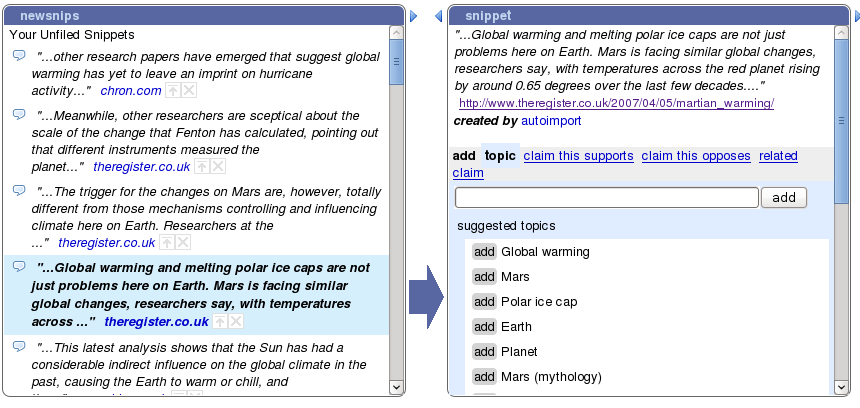
\includegraphics[width=8cm]{../screenshots/v2_sniptopic.png}
	\caption{Snippet first: Pick a claim or topic for each unfiled snippet}
	\label{sniptopic}
	\end{center}
\end{figure}

\item[Immediate:] A user can select a claim for a snippet that they have just marked. When a user marks a snippet, Think Link will initially highlight it in blue to show the user that the snippet is not currently associated with a claim or topic and will not be shown to other users. If the user clicks on the highlighted snippet, then Think Link will bring up the same suggestion panel used in the ``snippet first'' method.
\end{description}

When gathering ``interesting'' snippets, a user may want to associate a snippet with a general topic rather than a specific claim. It is only necessary to associate an ``interesting'' snippet with a claim when a user wants to offer support for a particular claim. In some cases a user will gather snippets that they might want to use later, but without concrete plans for how they might want to use them or what claims they might want to use them as evidence for. In such cases, it is easier to file the interesting snippets under a general topic and possibly attach them to a claim some time in the future. 

Think Link uses the Wikify! algorithm~\cite{Mihalcea2007} to suggest topics for snippets or claims. The Wikify algorithm imagines that a piece of text was on a Wikipedia pages and predicts what pages that text would be most likely to link to, based on the probability that any particular n-gram links to any particular page. Recall that the set of Think Link topics is seeded with the set of Wikipedia page titles. The Wikify algorithm performs significantly better than a word-frequency comparison as it biases towards topics that a heavily linked to.

\todo{Mention about topic previewing}

As the argument graph grows bigger it becomes increasingly important to make sure that it stays well connected. If different users are interested in the same topic then it is easy for them to create duplicate claims or not connect claims that should be connected. Think Link tries to make it easy for users to keep the claim graph well connected by suggesting claims that should be linked together.

\todo{Allow two claims to be marked as being identical}.


Think Link uses the same suggestion system to allow users to connect claims to snippets, and to connect claims to other related claims. 

\todo{BUG: don't have 'add' button for snippets}


\subsection{Implementation}

Think Link consists of a browser extension, a page annotation script, a shared public database of contentious claims, and a web-based argument interface that allows one to explore and manipulate the claim graph. These four components are largely independent of each other and talk to each other using an open API that can also be used by other tools. Indeed the settings panel for the browser extension allows a user to tell it to bind to alternative versions of the other modules.

The page annotation script is a javascript file that can be included into any HTML page. When it is run on a page it sends the page URL to the server, asking it to send back information about any contentious snippets on that page. If any such snippets are found, the page modification script highlights them in red. If the user clicks on a highlighted snippet then it shows an iframe containing a visualization from whatever visualization server it has been configured to use.

The only purpose of the browser extension is to insert the page modification script onto every page that the user loads. The browser extension is not the only way that one can access Think Link highlights. One can get the same effect by browsing through a proxy (like WBI~\cite{Barrett1997}), or if the owner of a web site included the page annotation script themselves.

Think Link's annotation system has some privacy issues. Every time the user browses to a page, the URL is sent to the Think Link server to check whether there are any known annotations for that page. Privacy issues are reduced by the fact that the requests contain no cookies or other identifying information, and can be cached by a third-party proxy if desired; however issues still remain. In future work hope to reduce these privacy issues. One possibility is to use a hashing system similar to that used by Google Safe Browsing\footnote{http://code.google.com/p/google-safe-browsing/}.

The protocol used by the Think Link server is an open REST API that other tools are free to use. We are also considering supporting one or more of the several argumentation interchange formats that have been proposed ~\cite{Rahwan2007a,McGinnis2007}.


\section{User Studies}

We performed two qualitative ``think aloud'' user studies. The aim of these studies was to inform the development of Think Link. The studies were not intended to validate the design of Think Link as being correct. Think Link is designed to be used by a large number of users gathering a vast amount of evidence for many different points. To confidently state that our design was successful we would need to be able to test Think Link on a much greater scale than we currently have resources for.

The aim of the first study was to see how users normally browse the web and see their reactions to an early version of the Think Link argument graph. The aim of the second study was to evaluate user responses to an updated version of the interface and evaluate how users responded to seeing highlighted snippets on the page. We present the results of the two studies together.

\subsection{Procedure for the First Study}

For the first study we recruited 12 paid participants. Five were female, seven were male. Their ages ranged from high school age to retired. Our intention was to recruit users who were not experts, but who regularly used the Internet to find information. We recruited participants using a posting to the Craigslist.org classified advert site. In our advert, we expressed an interest in people who use the Internet to gather knowledge, rather than just for tasks such as email or shopping. We filtered participants based on their short answers to questions about how they found, organized, and shared information on the web. 

\todo{This was a bad recruiting strategy. We should have recruited people that fitted one of our two personas and then set them tasks that fitted our vision for that persona.}

Study sessions took approximately 45 minutes. Participants were seated at a single-screen workstation with the Firefox browser augmented with the Think Link extension. We first demonstrated Think Link's interface, and then asked them to browse normally and use Think Link to identify snippets that made claims they thought were interesting or disputed and connect those claims to the existing claim graph. For the first half of the study, we asked them to constrain their browsing to political news articles, to increase the likelihood that there would be existing claims about the topic they were browsing.

In this initial study, users were exposed to the prototype interface shown in Figures~\ref{oldsnippetbox} and \ref{oldbrowser}, rather than the final interface described earlier in this paper. We discuss some of the key differences in the findings section.

\subsection{Procedure for the Second Study}

For the second study, we recruited 6 paid participants. Four were female and two were male. Although we recruited participants using the same advert as the first study, the timing of our second advert around the beginning of the college semester meant that five of the participants were students. Since the second group was different demographically to the first group, it was not possible to make a direct comparison between their behaviors. 

In the second study we were more confident about the usability of our tool and so we decided to tell them nothing about how to use it. We gave each user a brief introduction to the aims of the tool, similar to the introduction of this paper, and then asked them to perform two tasks with it. The first task was to look at a selection of web pages that already had highlighted snippets and explore the interface while thinking aloud about what they saw (the ``sceptical reader'' use case). The second task was to identify disputed claims on a set of pages we gave them about global warming and connect them appropriately to existing claims that we had pre-populated the claim graph with (the ``activist'' use case). 

Participants were shown the prototype interface shown in Figure~\ref{secondbrowser}. This is similar to the interface described earlier in this paper, but uses drag and drop to make connections, rather than a suggestion system.

\subsection{Findings}

In this section we present the findings from our two user studies. Findings from the two studies are presented together and clustered by topic.

\subsubsection{High-Level Impressions}

Response was generally positive, with many participants being very keen to use the tool soon. One participant said ``I can see myself getting addicted to this'', and several participants asked as to notify them when it is properly deployed. Most of the participants expressed an interest in using the tool, with some wanting to use it now, and others wanting to use it ``when it is more mature''.

Participants liked the ability to see when other pages disagreed with the claim they were looking at. One participant said ``The web needs to be taken with a grain of salt, and this gives you salt goggles''.

Most participants in the first study, and all participants in the second study were able to use the tool competently. Participants in the second study were able to use Think Link competently without it being demonstrated in advance and were able to correctly deduce what the different parts of the interface meant. Participants said they found the tool ``very intuitive''.

\subsubsection{Choosing a Claim for a Snippet}

\begin{figure}[t]
	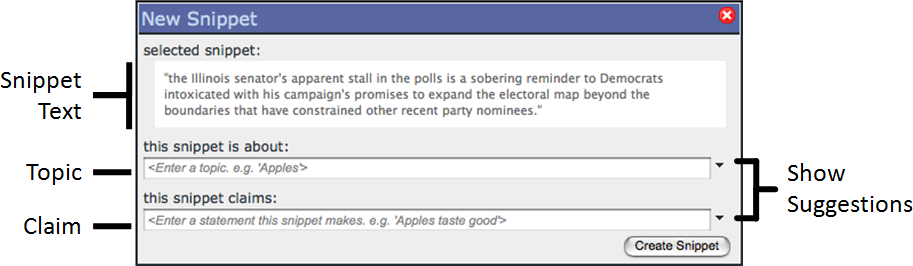
\includegraphics[width=8.5cm]{../screenshots/oldsnipcreate_diagram.png}
	\caption{First Prototype Snippet Creation Dialog}
	\label{oldsnippetbox}
\end{figure}

\begin{figure}[t]
\begin{center}
	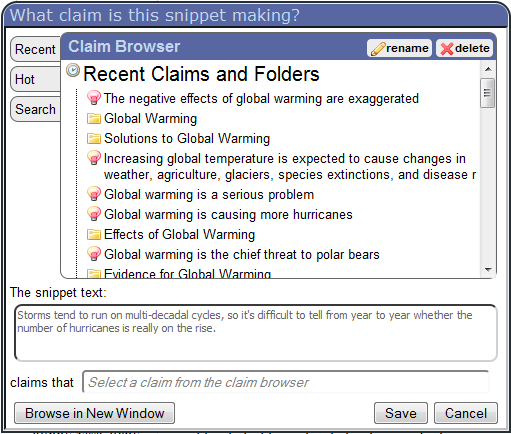
\includegraphics[width=5cm]{../screenshots/newsnip_browseopen.png}
	\caption{Second Prototype Snippet Creation Dialog}
	\label{secondsnippetbox}
\end{center}
\end{figure}

The prototype interfaces required that a user enter a claim for a snippet at the point at which they created the snippet. When the user marked a snippet, Think Link would display a dialog box asking them what claim to associate it with (Figure~\ref{oldsnippetbox} for the first prototype and Figure~\ref{secondsnippetbox} for the second prototype). There turned out to be several problems with requiring that a user select a claim at the point at which they marked a snippet:

Users would often encounter a snippet that could be interpreted as making several interesting claims. Users got confused by the need to pick only one claim. Some users dealt with this by writing a compound claim such as ``Global warming will cause X and Y'', while other users would mark several overlapping snippets making different claims. In the final interface one can associate a snippet with several claims.

Some users wanted to associate a snippet with a topic but without associating it with a specific claim. For example, they might find the text of an important speech, or the results of a sporting event. While it is possible that they might want to use this as evidence for a claim in the future, they didn't want to have to decide what the claim was immediately. In the final interface one can associate a snippet with a topic rather than a claim.

Some users seemed to be deterred from marking interesting snippets by the mental effort required to choose an appropriate claim. In several cases, we saw a user pause to decide whether an interesting snippet was worth marking up. Similarly, some users seemed to find it difficult to decide what the right claim to use for a snippet was, since they had not yet decided how they wanted to structure their argument, or even if this was a topic they wanted to argue about. The final interface does not require a user to associate a snippet with a claim at the time they create the snippet. Instead a user can mark snippets with minimal effort and then later search through their snippets to find evidence for particular claims.

Several users expressed confusion about how specific the claim made by a snippet should be, or when they should pick an existing claim rather than create a new one. For example, if a snippet says ``Global temperatures will rise by X degrees by 2050'' then is that making the claim ``Global temperatures will rise'', or should a new claim be created that contains the extra information? In the final interface, users can choose how specific to make their claims after they have gathered a large number of snippets and know what information is repeated between sources.

Since a user was required to enter a claim whenever they created a snippet, there was an incentive for the user to enter a claim as quickly as possible so they they could make the dialog go away. Several users created a new claim that was equivalent to a claim that already existed, and several users repeatedly created a claim that had the exact same text as the snippet. The final interface avoids this problem by allowing a used to delay the association of a claim for a snippet until they know what useful claim they want to use that snippet as evidence for.

\todo{Need to do some kind of evaluation to show that the new interface solves these problems}


\subsubsection{Choosing what to mark as a snippet}

Many users would consistently mark the first paragraph of an article as a snippet. This paragraph would frequently summarize the arguments made in the rest of the document document and often made an important claim that other claims in the document supported or provided context for. 

Several users wanted to mark up a table or an image as a snippet. This is valid behavior -- a table or image is often useful evidence for a claim; however it is not currently supported by Think Link. In future versions of Think Link we intend to support this behavior.


\subsubsection{Connecting Claims}

Many participants expressed a desire to organize claims into connected arguments during their session. 

Some users incorrectly marked one claim as supporting another when in fact they should have both been marked as supporting a third claim that needed to be created. For example ``Global warming is causing more hurricanes'' does not support ``Global warming is causing rising sea levels'', but both support ``Global warming is causing environmental problems''. Users realized that the claims were related, but did not immediately recognize that they needed to create new claims in order to structure the relationship correctly. It is possible that creating correct logical claim structures may just be too difficult for some people, or it may be that users would get used to the idea with more practice. We hope that if Think Link was deployed more widely many of the intermediate claims that were needed would already have been created and this problem would thus be reduced.

Some users were confused by claims that had a ``because'' relationship rather than a ``supports'' or ``opposes'' relationship. For example ``America did not sign the Kyoto Protocol'' {\it because} ``Signing Kyoto would harm the US economy''. Similarly, many users expressed a desire to mark claims as being ``related'' without supporting or opposing each other. For example ``America did not sign the Kyoto Protocol'' {\it is related to} ``America was right to not sign the Kyoto Protocol''. In the first prototypes, a user needed to chose between ``supports/opposes'' when connecting two claims together (following gIBIS~\cite{Conklin1987a}). In the final interface we introduced a ``related-to'' link type to allow users to connect claims that they thought should be related but which didn't confirm to a simple pro/con relationship. 

Several users got confused by claims that referred to similar events at different points in time. For example, one participant in the first study marked a two claims as opposing each other when each was true at the time that it was written. This is a particular problem when talking about breaking news events, where what claims are true can change fast. If Think Link is to be effective for describing such events then it is likely that it will need to have better support for identifying the time at which a claim was asserted to be true.

Several users expressed an interest in being able to mark a claim as controversial without having to create an opposing claim. One user said that opposing a claim required ``too many clicks'' and they wanted to be able to just vote against a claim without having to say why or find evidence. In the future we are planning to implement a social voting system to allow users to say what claims they believe are false and see what claims their friends agreed or disagreed with.

\begin{figure}[tb]
	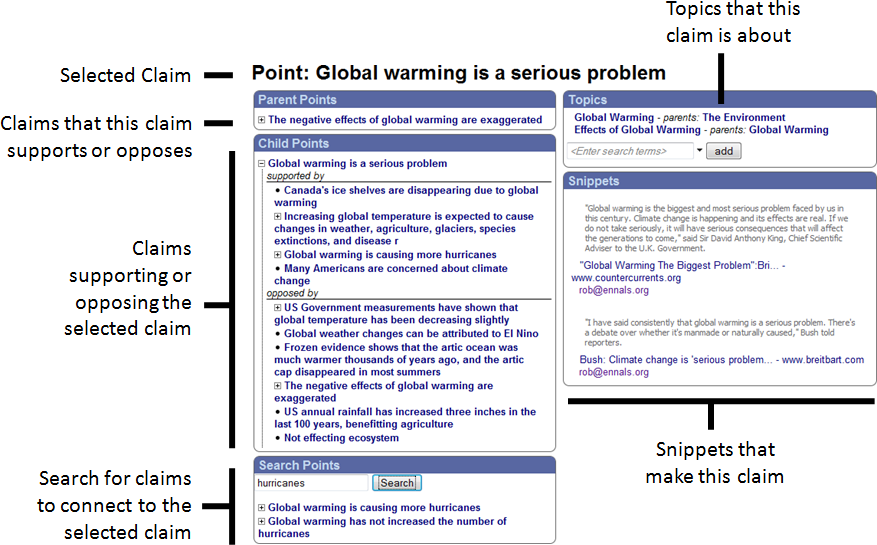
\includegraphics[width=8.5cm]{../screenshots/oldpoint_diagram.png}
	\caption{First Prototype Claim Browser}
	\label{oldbrowser}
\end{figure}

\begin{figure}[tb]
\begin{center}
	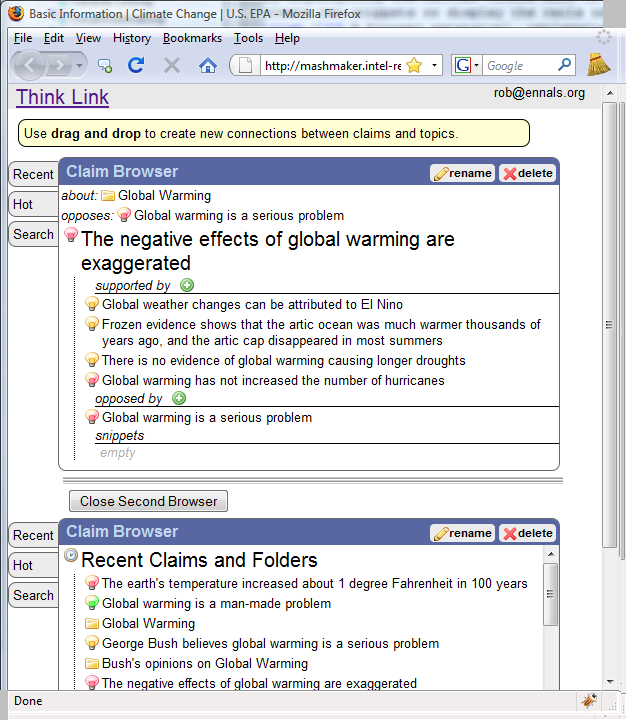
\includegraphics[width=5cm]{../screenshots/claimbrowse.png}
	\caption{Second Prototype Claim Browser}
	\label{secondbrowser}
\end{center}
\end{figure}

The first two versions of Think Link used a drag-and-drop interface to allow a user to create links between claims. In the first interface (Figure~\ref{oldbrowser}) a user could use a search box to find other claims and then drag them into an appropriate position in the argument tree. In the second interface (Figure~\ref{secondbrowser}), followed a file-manager metaphor, providing two identical browser windows that a user could drag and drop claims between. In both cases, we found that users would often not intially realize they could use drag and drop to organize claims, even when we added a prominent information message at the top of the display (Figure~\ref{secondbrowser}). We believe that part of the problem was that users are not used to using drag-and-drop in a web interface, and there was no visible clue in the rendering of the claim graph that they could use drag and drop to create connections. In the final interface we resolved this issue by having the connection actions (``add claim'' etc) explicitly visible in the interface.

\section{Future Work}

At present Think Link relies on users to mark up snippets and connect them to claims. In the future we plan to explore using natural language and machine learning techniques to assist in this process. Our plan is to allow a user to request that Think Link present them with potential web snippets that make a claim that they disagree with, and then quickly select which of these should be highlighted as being contentious.

Think Link is designed to be used as a social tool in which large numbers of people collaborate to find large numbers of claims and snippets about interesting topics. Since our graph and user base are currently small, we have not yet evaluated how Think Link works when data sets are huge, many users are concurrently editing data, and some users are malicious.

We think it could be useful to use Think Link as a tool to suggest reading material. Just as tools like Digg suggest pages that you might like, Think Link could potentially suggest pages that contain claims that the user had not read and would be likely to find interesting.

\section{Conclusions}

We have introduced the idea of enhancing the browsing interface by highlighting snippets of text that make disputed claims and allowing a user to see an argument graph that presents the best evidence on either side of the issue. Think Link allows users to navigate between pages based on the factual claims made on pages, rather than being restricted to the links provided by authors. It allows users to identify disputed claims on web pages and connect them directly to the arguments that those claims are part of, and related claims on other web sites.

On a practical level, Think Link works by allowing users to pick out snippets on pages that make claims that they think are interesting or controversial, and then using a collaborative filtering model to allow users to vote for the most interesting evidence and structure claims into a coherent argument graph.

We hope that Think Link will make it easier for people to be informed about the world and be exposed to factual claims that they might not otherwise be exposed to.

\section{Acknowledgments}

Acknowledgements omitted for blind submission. Think Link uses icons from the free FamFamFam Silk\footnote{http:\\famfamfam.com} collection.


\todo{Sort out bad references}
\bibliography{refs}

\end{document}



